\documentclass{standalone}
\usepackage{graphicx}	
\usepackage{amssymb, amsmath}
\usepackage{color}

\usepackage{tikz}
\usetikzlibrary{calc, arrows.meta}
\usepackage{pgfmath}

\definecolor{light}{RGB}{220, 188, 188}
\definecolor{mid}{RGB}{185, 124, 124}
\definecolor{dark}{RGB}{143, 39, 39}
\definecolor{highlight}{RGB}{180, 31, 180}
\definecolor{gray10}{gray}{0.1}
\definecolor{gray20}{gray}{0.2}
\definecolor{gray30}{gray}{0.3}
\definecolor{gray40}{gray}{0.4}
\definecolor{gray60}{gray}{0.6}
\definecolor{gray70}{gray}{0.7}
\definecolor{gray80}{gray}{0.8}
\definecolor{gray90}{gray}{0.9}
\definecolor{gray95}{gray}{0.95}

\newcommand*{\offset}{0.025}

\begin{document}

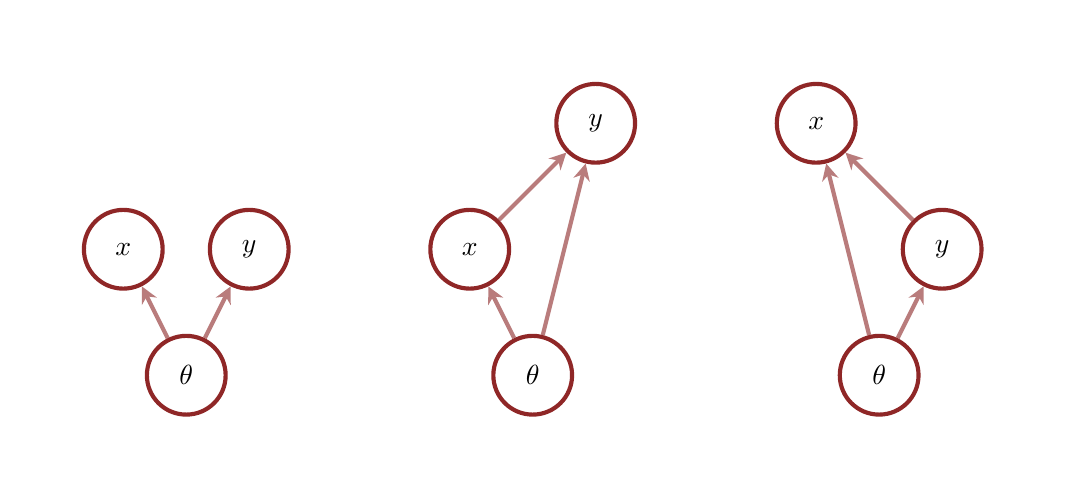
\begin{tikzpicture}[scale=0.2, thick]

  \pgfmathsetmacro{\r}{2.5}
    
  \begin{scope}[shift={(0, 0)}]  
    \draw[white] (-14, 2) rectangle (6, 30);

    \coordinate (C) at (-4, 8);
    \coordinate (D) at (-8, 16);
    \coordinate (F) at (0, 16);
  
    \foreach \B/\E in {C/D, C/F} {
      \draw[-{Stealth[length=6pt, width=6pt]}, shorten <=15, shorten >=15, color=mid, line width=1.5] (\B) -- (\E);
    }
  
    \filldraw[fill=white, draw=dark, line width=1.5] (C) circle (\r)
    node[color=black] { $\theta$ };
  
    \filldraw[fill=white, draw=dark, line width=1.5] (D) circle (\r)
    node[color=black] { $x$ };
  
    \filldraw[fill=white, draw=dark, line width=1.5] (F) circle (\r)
    node[color=black] { $y$ };
  \end{scope}
  
  \begin{scope}[shift={(22, 0)}]  
    \draw[white] (-14, 2) rectangle (6, 30);

    \coordinate (C) at (-4, 8);
    \coordinate (D) at (-8, 16);
    \coordinate (F) at (0, 24);
  
    \foreach \B/\E in {C/D, C/F, D/F} {
      \draw[-{Stealth[length=6pt, width=6pt]}, shorten <=15, shorten >=15, color=mid, line width=1.5] (\B) -- (\E);
    }
  
    \filldraw[fill=white, draw=dark, line width=1.5] (C) circle (\r)
    node[color=black] { $\theta$ };
  
    \filldraw[fill=white, draw=dark, line width=1.5] (D) circle (\r)
    node[color=black] { $x$ };
  
    \filldraw[fill=white, draw=dark, line width=1.5] (F) circle (\r)
    node[color=black] { $y$ };
  \end{scope}
  
  \begin{scope}[shift={(44, 0)}]  
    \draw[white] (-14, 2) rectangle (6, 30);

    \coordinate (C) at (-4, 8);
    \coordinate (D) at (-8, 24);
    \coordinate (F) at (0, 16);
  
    \foreach \B/\E in {C/D, C/F, F/D} {
      \draw[-{Stealth[length=6pt, width=6pt]}, shorten <=15, shorten >=15, color=mid, line width=1.5] (\B) -- (\E);
    }
  
    \filldraw[fill=white, draw=dark, line width=1.5] (C) circle (\r)
    node[color=black] { $\theta$ };
  
    \filldraw[fill=white, draw=dark, line width=1.5] (D) circle (\r)
    node[color=black] { $x$ };
  
    \filldraw[fill=white, draw=dark, line width=1.5] (F) circle (\r)
    node[color=black] { $y$ };
  \end{scope}
  
\end{tikzpicture}

\end{document}  